%%%%%%%%%%%%%%%%%%%%%%%%%%%%%%%%%%%%%%%%%%%%%%%%%%%%%%%%%%%%%%%%%%%%%%
% How to use writeLaTeX: 
%
% You edit the source code here on the left, and the preview on the
% right shows you the result within a few seconds.
%
% Bookmark this page and share the URL with your co-authors. They can
% edit at the same time!
%
% You can upload figures, bibliographies, custom classes and
% styles using the files menu.
%
%%%%%%%%%%%%%%%%%%%%%%%%%%%%%%%%%%%%%%%%%%%%%%%%%%%%%%%%%%%%%%%%%%%%%%

\documentclass[12pt]{article}
\usepackage{sbc-template}

\usepackage{graphicx,url,xcolor,enumerate}
\usepackage{placeins}
\usepackage{float}

\usepackage[brazil]{babel}   
\usepackage{titlesec}
\usepackage[utf8]{inputenc}  

\sloppy

\title{Caracterização dos Domínios de Repositórios do Github Dependentes das Tecnologias Electron e Windows Forms}

\author{Guilherme Gabriel S. Pereira, Henrique P. F. Monteiro, Lucas Ângelo O. M. Rocha, 
\\ Victor B. G. Campos, Vinícius M. C. e Oliveira, Professor Felipe Augusto Lima Reis, 
\\ Professor José Laerte Pires Xavier Junior }

\address{
    Unidade Praça da Liberdade \\ 
    -- Pontifícia Universidade Católica de Minas Gerais (PucMinas) \\
    -- Belo Horizonte -- MG -- Brazil \\
    Departamento de Engenharia de Software e Sistemas de Informação \\
    -- PucMinas -- Belo Horizonte, MG.
    \email{\{ggspereira,laomrocha,henrique.forte,}
    \email{vinicius.marini,vbgcampos\}@sga.pucminas.br}
    \email{\{falreis,laertexavier\}@pucminas.br}
}

\begin{document} 

\maketitle 

\begin{abstract}

  Electron and Windows Forms are technologies used to create \textit{software} for the \textit{desktop} platform. Managers of new projects and systems analysts, when intending to develop an application for the \textit{desktop} platform, may be curious to know if their application domain is popular. Therefore, this work aims to characterize Github repositories dependent on Electron and Windows Forms technologies and their respective domains, with respect to their metrics by domains and popularity, in the context of Github repositories that have application dependencies \textit{desktop} of JavaScript and C\# languages. For this, a search was made of 1.781 repositories that fit these requirements, to analyze through artificial intelligence, which were the respective domains of these repositories. With this, the main domains of these repositories were found, namely, \textit{Library} and \textit{Framework}, followed by domains related to screen image capture (\textit{Screen Recorder}, \textit{Screen Sharing} and \textit{Screen Capture}) and editors. It was also possible to identify that the number of repositories has been decreasing in recent years, and had its peak in 2016. On the other hand, community engagement has shown growth over the years.

\end{abstract}
     
\begin{resumo} 

  Electron e Windows Forms são tecnologias utilizadas para criar \textit{software} para a plataforma \textit{desktop}. Gestores de novos projetos e analistas de sistemas ao pretenderem desenvolver uma aplicação para a plataforma \textit{desktop} podem ter a curiosidade de saber se o domínio da aplicação deles possui popularidade. Diante disso, este trabalho tem como objetivo caracterizar repositórios do Github dependentes das tecnologias Electron e Windows Forms e seus respectivos domínios, com relação às suas métricas por domínios e popularidade, no contexto dos repositórios do Github que possuem dependências de aplicações \textit{desktop} das linguagens JavaScript e C\#. Para isso, foi feita uma busca de 1.781 repositórios que se encaixavam nestes requisitos, para analisar, por meio de inteligência artificial, quais eram os respectivos domínios destes repositórios. Com isso, foi encontrado os principais domínios desses repositórios, sendo eles, \textit{Library} e \textit{Framework}, seguidos dos domínios relacionados a captura de imagem de tela (\textit{Screen Recorder}, \textit{Screen Sharing} e \textit{Screen Capture}) e editores. Foi possível identificar também que o número de repositórios vêm diminuindo nos últimos anos, e teve seu pico em 2016. Em contrapartida, o engajamento da comunidade tem apresentado crescimento ao longo dos anos.

\end{resumo}


\section{Introdução} \label{introducao}

Um desafio atual para empresas desenvolvedoras de \textit{software} e analistas de sistemas independentes é escolher entre plataformas \textit{web}, \textit{mobile} e \textit{desktop} para suas aplicações, visando atrair com mais eficácia seus usuários~\cite{9463138}. O sucesso de um novo produto de \textit{software} está relacionado com sua forma disponibilização ao público, consequentemente ligado a qual plataforma ele está disponível~\cite{9463138}. Deve-se ressaltar que um mesmo \textit{software} não está restrito a apenas uma plataforma, mas é recomendável uma análise de viabilidade econômica antes de disponibilizar em alguma plataforma~\cite{Eke2019}. Diante disso, durante essa análise feita por empresas e desenvolvedores, há o problema de definir se é conveniente implementar uma solução do \textit{software} feito com as dependências Electron e Windows Forms para a plataforma \textit{desktop}, sendo necessário saber os domínios mais populares e corriqueiros dos repositórios desenvolvidos para \textit{desktop} com Electron e Windows Forms na atualidade e se são compatíveis com os domínios do \textit{software} em análise.

O problema a ser solucionado nesta pesquisa é a carência de um estudo específico que busque analisar e classificar os objetivos mais comuns dos Repositórios do Github Dependentes das Tecnologias Electron e Windows Forms (RGDTEW). A partir desta pesquisa, tem-se um estudo no qual é possível compreender quais são os domínios mais recorrentes e as popularidades destes domínios no contexto de aplicações desenvolvidas com as tecnologias Electron e Windows Forms. As tecnologias Electron e Windows Forms são utilizadas para desenvolver sistemas para a plataforma \textit{desktop} nas linguagens de programação JavaScript e C\#. Os domínios são definidos como os adjetivos que definem os objetivos que o repositório se propõe, como, por exemplo, repositórios de aplicações \textit{desktop} que buscam detectar e eliminar vírus, são definidos no domínio antivírus.

A motivação que levou desenvolver-se esta pesquisa é compreender melhor o cenário atual dos RGDTEW, se ele esta em fase de crescimento ou não, após o aumento no uso de aplicações \textit{web} e \textit{mobile}, fortemente influenciado pela pandemia da COVID-19~\cite{KATSUMATA2022100168}. Busca-se adquirir um maior conhecimento sobre os sistemas desses repositórios, seus domínios e popularidades das aplicações Electron e Windows Forms. 

Assim, o trabalho justifica-se, porque desenvolvedores, gestores e analistas de sistemas podem analisar estas informações e decidirem se compensa desenvolver seu produto para a plataforma \textit{desktop} em Electron ou Windows Forms, conforme o nível de popularidade do domínio. Desta forma, este estudo auxilia os responsáveis por produtos de \textit{software} a implementar aplicações para os domínios populares no contexto \textit{desktop} nas linguagens de programação JavaScript e C\#, por meio da caracterização dos principais domínios dos RGDTEW da atualidade.

Este trabalho tem como objetivo geral explorar e caracterizar os RGDTEW e seus respectivos domínios, com relação às suas métricas de popularidade e por domínios, do ponto de vista de analistas, gerentes e clientes de novos projetos, no contexto dos repositórios do Github que possuem dependência das tecnologias Electron e Windows Forms. Desta forma, para alcançar resultados, foram delimitados objetivos específicos, por meio das seguintes três questões de pesquisa e suas respectivas métricas:

\begin{enumerate}
  \item[QP.1] Para os RGDTEW, qual o domínio que elas se encontram atualmente?
    \begin{enumerate}
        \item[M.1] Proporção de repositórios que possuem descrições e domínios contra que não possuem descrições ou domínios;
        \item[M.2] Percentual da quantidade de dependentes das tecnologias Electron e Windows Forms para cada domínio.
    \end{enumerate}
  \item[QP.2] A quantidade dos RGDTEW vem diminuindo ao longo da última década?
    \begin{enumerate}
        \item[M.3] Média dos RGDTEW criados por ano para cada domínio;
        \item[M.4] Média dos RGDTEW criados por ano.
    \end{enumerate}
  \item[QP.3] Os RGDTEW tem engajamento da comunidade?
    \begin{enumerate}
        \item[M.5] Percentual de \textit{pull requests merged} em relação aos não \textit{merged} dos RGDTEW por ano;
        \item[M.6] Percentual de \textit{issues} fechadas em relação a não fechadas dos RGDTEW por ano.
    \end{enumerate}
\end{enumerate}

A organização do conteúdo a seguir deste trabalho se define da seguinte forma: na Seção \ref{trabalhosrelacionados} são caracterizados os trabalhos relacionados; a Seção \ref{metodologia} aborda as técnicas utilizadas para responder às questões formuladas; na Seção \ref{resultados} são apresentados os resultados encontrados para responder às questões da pesquisa; a Seção \ref{discussao} tem-se a discussão sobre os resultados obtidos; na Seção \ref{ameacas} são apresentadas as ameças à validade de conclusão, construção, internas e externas; a Seção \ref{conclusao} apresenta uma conclusão do estudo.

\section{Trabalhos Relacionados} \label{trabalhosrelacionados}

Nesta seção são abordados os artigos encontrados na literatura, usados para guiar a pesquisa do presente trabalho. Os artigos analisados descrevem, respectivamente, um método de caracterização de aplicações, as tecnologias web para desenvolvimento desktop, o crescente aumento do uso de dispositivos móveis, métricas para escolha de repositórios e o método de inteligência artificial utilizado para a caracterização de repositórios na pesquisa. 

Sobre a caracterização de aplicações, ~\cite{4561878} descreve como objetivo investigar a viabilidade do uso de técnicas não supervisionadas para a classificação taxonômica de aplicações \textit{desktop}, ou seja, o domínio de determinada aplicação, com base nos \textit{logs} gerados pelas aplicações. Para tal, foram utilizados dois métodos diferentes: análise de co-ocorrência e análise de cluster. Foi concluído que ambas abordagens produziam um resultado com acurácia satisfatória. O método de classificação se difere do apresentado no presente trabalho, pois este não necessita da execução do sistema para efetuar a classificação.

Tratando das tecnologias de plataforma \textit{desktop}, o estudo realizado por~\cite{toman2019depth} comparou os principais \textit{frameworks} de \textit{software} para desenvolvimento dessas aplicações usando tecnologias da \textit{web}, Electron e NW.js, por um estudo de caso e uma análise de conteúdo, comparando diversas características entre os \textit{frameworks}, como arquitetura, ferramentas para construir a interface com o usuário, e facilidade de integração com sistemas. Levantando todos os prós e contras dos \textit{frameworks}, o Electron se mostrou como o mais adequado, principalmente no que diz respeito à integração de sistemas, a interface com o usuário, sistema de arquivos e funcionalidades multimídia. Esse artigo contribui para a escolha do Electron como tecnologia a ser pesquisada no presente trabalho.

Utilizando de um estudo de caso, ~\cite{KATSUMATA2022100168} realiza uma análise das mudanças do uso de dispositivos móveis durante a pandemia do COVID-19. Mais especificamente, o estudo coletou dados de utilização dos dispositivos no Japão, analisando os períodos do primeiro e segundo pico do coronavírus. O objetivo desse artigo foi analisar as mudanças no uso de dispositivos móveis durante a crise do COVID-19. Os autores concluem que o uso de dispositivos móveis aumentou significativamente durante a pandemia, com as pessoas se voltando para eles para se manter conectadas e informadas. Considerando esse aumento, a pesquisa contribui para um dos questionamentos proposto no presente trabalho, de que estaria havendo uma diminuição da popularidade dos RGDTEW, no geral.

Em relação às métricas escolhidas, o estudo de ~\cite{9282287} visa entender quais métricas devem ser usadas para buscar repositórios em pesquisas científicas para diversos casos. O trabalho faz a análise de diversos repositórios, alterando os critérios de busca. Alguns destaques encontrados na pesquisa são o uso de número de contribuidores do repositório e busca por dependências. Neste contexto, o artigo foi utilizado para discussão de quais critérios deveriam ser usados na escolha dos repositórios a serem analisados.

Sobre o método classificatório, o trabalho de ~\cite{radford2018improving} apresenta o Pré-Treinamento Generativo (GPT, do inglês \textit{Generative Pre-Training}), o método usado para treinar modelos de linguagem. O método se baseia em uma etapa de pré-treinamento não supervisionado, seguido de uma etapa de ajuste fino, ou afinação. Os testes demonstraram que este \textit{framework} consegue produzir modelos capazes de executar diversas tarefas de processamento de linguagem natural, como responder a perguntas, tarefas de similaridade semântica e classificação. O modelo descrito é usado no presente trabalho, mais especificamente, para a tarefa de classificação de domínios dos repositórios.

\section{Metodologia} \label{metodologia}

Esta pesquisa tem como escopo buscar projetos \textit{open-source} no Github que são dependentes das tecnologias Electron e Windows Forms e validar se seus domínios ainda possuem popularidade. Para esse propósito foram coletadas as descrições, \textit{pull requests} e \textit{issues} de repositórios mais populares das linguagens C\# e Javascript, que possuíam alguma dependência das tecnologias \textit{desktop} Electron e Windows Forms. 

O processo de análise está dividido em cinco etapas, ilustrado na Figura \ref{fig:Metodologia} e explicitado a seguir: 1. Coleta de repositórios; 2. Recolhimento de \textit{issues} e \textit{pull requests}; 3. Análise de domínio utilizando inteligência artificial; 4. Filtragem manual de domínios; 5. Reavaliação de repositórios com domínios definidos. Para a realização das etapas, com exceção da quarta, foram criados \textit{scripts} na linguagem Python para realizar a coleta e processamento de dados, salvos em um banco de dados relacional local.

\begin{figure}[ht]
    \centering
    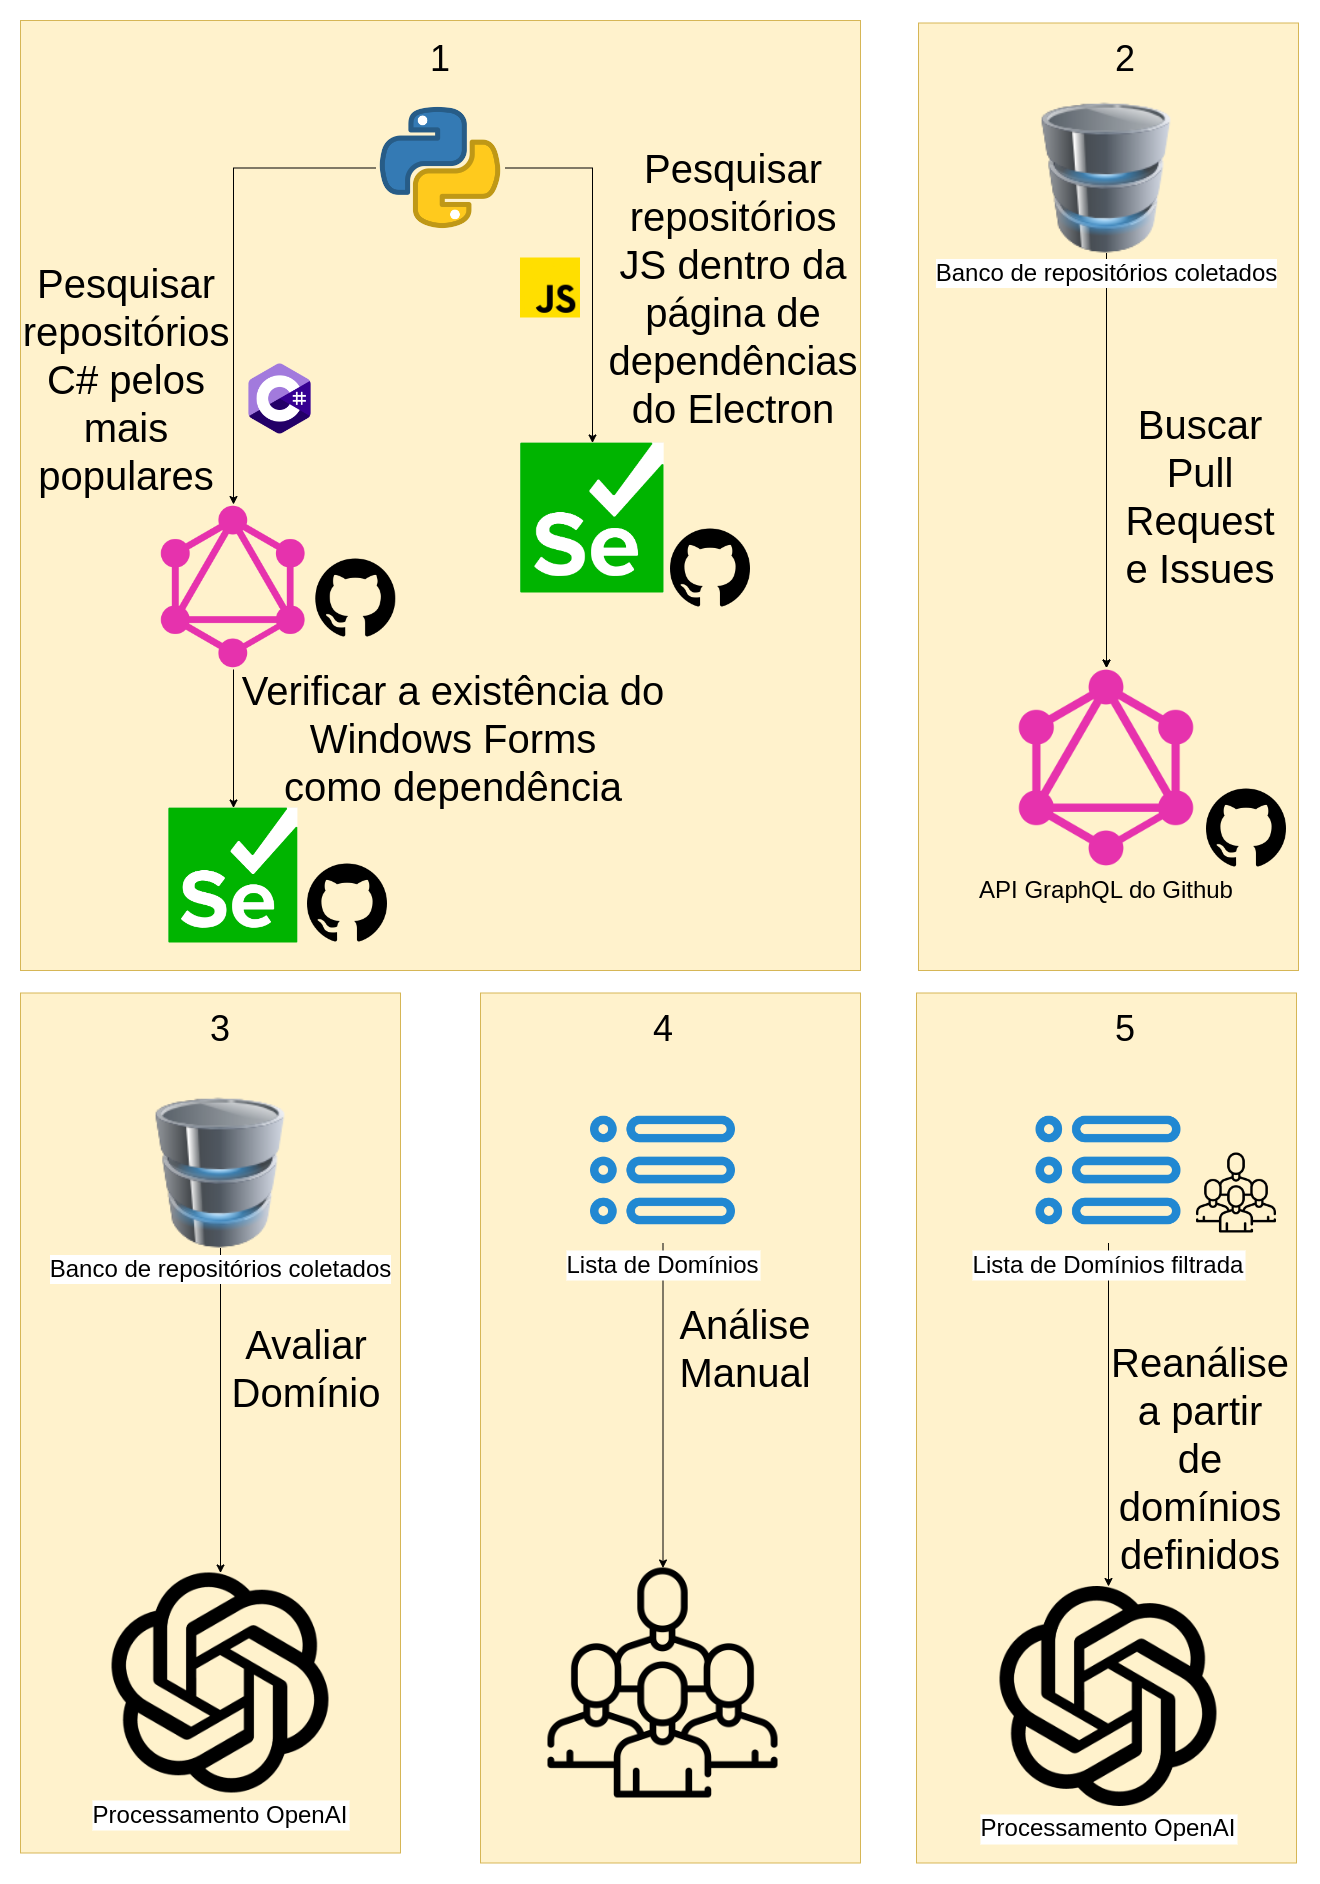
\includegraphics[width=0.7\textwidth]{images/metflow222.png}
    \caption{Ilustração das etapas da metodologia adotada}
    \label{fig:Metodologia}
\end{figure}

\subsection{Etapas da metodologia}

Nesta seção são apresentadas as cinco etapas, presentes na Figura \ref{fig:Metodologia}, utilizadas neste estudo exploratório de caracterização de domínios dos RGDTEW e suas popularidades. Essa seção foi construída visando descrever os processos utilizados para coletar e processar os dados utilizados em nossa análise de resultados.

Na Etapa 1, para realizar o filtro de quais repositórios estavam na categoria \textit{desktop} foram utilizados dois procedimentos, um para cada linguagem de programação. No primeiro procedimento, para a busca de repositórios em C\#, foi utilizada à interface de programação de aplicação (API, do inglês: \textit{Application Programming Interface}) de GraphQL disponibilizada pela plataforma Github. Por meio dessa interface, realizou-se uma busca ordenada pelos repositórios mais populares, conforme o número de estrelas~\cite{DBLP:journals/corr/abs-1811-07643}, os quais verificou-se que o \textit{software} era construído utilizando Windows Forms (estrutura para criação de aplicativos da área de trabalho do Windows da linguagem C\#) por meio do grafo de dependência. O segundo procedimento buscou todos os repositórios que utilizavam o Electron (\textit{framework} para construir aplicações \textit{desktop} usando Javascript, Linguagem de Marcação de Hipertexto (HTML, do inglês: \textit{HyperText Markup Language}) e Folha de Estilos em Cascata (CSS, do inglês: \textit{Cascading Style Sheets}), utilizando seu grafo de dependência.

Em seguida, para realizar a busca das dependências do projeto utilizou-se o Selenium, uma ferramenta de automação de testes para aplicações \textit{web}. A ferramenta foi utilizada para auxiliar a realizar uma busca nos grafos de dependência dos repositórios, disponível na plataforma do Github, devido API de GraphQL do Github não possuir essa funcionalidade.

Sequencialmente, na Etapa 2, utilizando a lista de repositórios encontrada, foram coletados por meio da interface GraphQL do Github todos os \textit{pull requests} e \textit{issues} dos repositórios das duas linguagens recolhidos. O estudo considerou 1.781 repositórios coletados no período de setembro a outubro de 2022, sendo 561 repositórios com mais de 300 estrelas em C\# e outros 1220 que possuem mais de 1000 estrelas feitos em Javascript

A Etapa 3, no que lhe concerne, utilizou os repositórios obtidos na etapa anterior na plataforma de inteligência artificial denominada OpenAI, visando realizar a leitura de descrição de cada repositório e definir um domínio para ele. Esse processo atribuiu 604 domínios únicos para os 1.781 repositórios, sendo que 395 repositórios foram descartados.

Posteriormente, na Etapa 4, a lista dos 604 domínios passou por uma análise manual, para que domínios que possuem semelhanças como: termos no plural e palavras semelhantes com apenas uma ocorrência fossem removidos e reavaliados novamente. Ao final da análise manual foram selecionados 68 domínios únicos, utilizados para efetuar uma nova atribuição pela inteligência artificial.

A Etapa 5 culminou na reavaliação dos repositórios por meio da OpenAI, utilizando os 68 domínios para decidir qual era o mais próximo da descrição, podendo também não definir nenhum caso julgasse fora do escopo do repositório ou caso não houvesse uma descrição definida. A análise dos dados como \textit{pull requests}, \textit{issues} e domínios desses repositórios definidos como fora de escopo foi realizada separadamente dos demais repositórios, para que não houvesse influência nos resultados.

\subsection{Hipóteses e Métricas}

Nestas seções serão discorridas as questões de pesquisa, suas respectivas métricas e as hipóteses levantadas. Hipóteses são suposições construídas para guiar a tomada de decisão. Métricas são medidas usadas para monitorar e avaliar o desempenho da pesquisa. Essas métricas ajudam a identificar tendências, problemas e oportunidades. Elas também fornecem uma visão geral dos resultados esperados e dão \textit{feedback} sobre as hipóteses criadas.

\subsubsection{QP.1 Para os RGDTEW, qual o domínio que elas se encontram atualmente?}

Mediante ao cenário atual de popularização das tecnologias \textit{web}, a decisão do tipo de plataforma em que um \textit{software} deverá ser disponibilizado  deverá considerar uma série de fatores. Um desses fatores é se o domínio do \textit{software} convém ser disponibilizado em plataforma \textit{desktop} atualmente. Sendo assim, foi levantada a QP.1.

Para responder essa questão, foram definidas 2 métricas. A métrica M.1 (Proporção de repositórios que possuem descrições e domínios contra que não possuem descrições ou domínios) visa exibir a quantidade de RGDTEW que declararam sobre o que se trata seu \textit{software}. A métrica M.2 (Percentual da quantidade de dependentes das tecnologias Electron e Windows Forms para cada domínio) tem como objetivo identificar os principais domínios cujas aplicações \textit{desktop} feitas com Electron e Windows Forms ainda são utilizadas e consequentemente haverá sentido disponibilizar uma versão \textit{desktop} desenvolvida com Electron ou Windows Forms de uma aplicação dentro desses domínios. 

A hipótese inicial é de que os principais domínios seriam voltados para aplicações de antivírus, editores de imagens e vídeos, compartilhamento de tela, pois essas aplicações exigem maior contato com os recursos do hardware, levando vantagem em ser utilizadas via \textit{desktop}.

\subsubsection{ QP.2 A quantidade dos RGDTEW vem diminuindo ao longo da última década? }

Um fator que é de suma importância para manutenção do \textit{software} é saber se a tecnologia escolhida terá longevidade, ao passo que escolher uma tecnologia no qual a tendência é a depreciação resultará em empecilhos na evolução e manutenabilidade do \textit{software}~\cite{7965364}. Dado este fato, foi levantada a nossa segunda questão de pesquisa, a QP.2.

Para responder essa questão, foram definidas 2 métricas. A métrica M.3 (Média dos RGDTEW criados por ano para cada domínio) e a métrica M.4 (Média dos RGDTEW criados por ano). O objetivo dessas métricas é exibir a tendência de RGDTEW dos últimos anos para cá, seja por um domínio específico ou não. Dado a popularização e o crescimento de tecnologias \textit{web}, é provável que haja tendência de queda para os RGDTEW de 2018 até a atualidade.

\subsubsection{QP.3 Os RGDTEW tem engajamento da comunidade?}

A comunidade de uma tecnologia é outro fator importante para definir a arquitetura do \textit{software}, pois ao surgirem dúvidas ou problemas durante o desenvolvimento de um \textit{software} é de suma importância que existam usuários engajados na comunidade que passaram por algo semelhante e podem ajudar a lidar com esse problema~\cite{9282287}. Isto posto, foi levantada a nossa terceira questão de pesquisa, a QP.3.
 
Para responder essa questão, foram definidas 2 métricas. A métrica M.5 (Percentual de \textit{pull requests merged} em relação aos não \textit{merged} dos RGDTEW por ano) para ilustrar cronologicamente a contribuição da comunidade quanto a \textit{software} \textit{desktop} das linguagens JavaScript e C\#. Dado a popularização e o crescimento de tecnologias \textit{web}, é possível que haja uma tendência de queda para os \textit{pull requests} de RGDTEW de 2018 até a atualidade. 

A métrica M.6 (Percentual de \textit{issues} fechadas em relação a não fechadas dos RGDTEW por ano) com o propósito de mostrar se os problemas relatados vêm sendo resolvidos durante os anos. Dado a popularização e o crescimento de tecnologias \textit{web}, possivelmente há uma queda na quantidade de \textit{issues} de repositórios dependentes das tecnologias Electron e Windows de 2018 até a atualidade.

\subsection{Análise de resultados} 

Os dados coletados na etapa de mineração passaram por tratamentos via MySQL que possibilitou a extração das quantidades de repositórios agrupados por domínio, \textit{issues}, \textit{pull requests} e os anos. Em seguida os dados foram exportados para planilhas do \emph{Google Sheets}, ferramenta de planilhas na \textit{web}, utilizada para adequar os dados e posteriormente importar a planilha ajustada no \emph{Google DataStudio}, ferramenta do Google que foi utilizada para a geração dos relatórios e painéis informativos que possibilitaram uma análise visual dos resultados descritos na Seção \ref{resultados}.

\section{Resultados} \label{resultados}

Após realização de todo processo descrito na metodologia e análise dos dados coletados, os seguintes resultados para responder às questões de pesquisa (QP.1, QP.2 e QP.3). Foram utilizadas as métricas definidas (M.1, M.2, M.3, M.4, M.5 e M.6) para calcular os resultados.

\subsection{QP.1 Para os RGDTEW, qual o domínio que elas se encontram atualmente?}

Em vista da métrica M.1 (Proporção de repositórios que possuem descrições e domínios contra que não possuem descrições ou domínios), referente a QP.1, que consiste na proporção entre repositórios que possuem descrições e domínios e repositórios que não possuem descrições ou domínios, foram encontrados os dados descritos na Tabela \ref{tab:descricao x sem descricao}{}.
\begin{table}[ht]
    \caption{RGDTEW com e sem domínio definido}
    \centering
    \label{tab:descricao x sem descricao}
        \begin{tabular}{|l|l|l|}
        \hline
        Repositório & Quantidade & Percentual\\
        \hline
        Sem domínio ou sem descrição & 395 & 22.17\%\\
        \hline
        Com domínio & 1.386 & 77.83\%\\
        \hline
        \end{tabular}
\end{table}
Dos 1.781 repositórios coletados, foi possível definir domínios, com o auxílio da ferramenta \emph{OpenAI}, os repositórios que possuem descrição e domínio (77.83\%) e os que não possuem (22.17\%). Os repositórios que não tiveram as descrições encontradas foram os que não possuíam o campo \emph{description} em suas páginas do Github e também outros que a inteligência artificial não obteve sucesso ao tentar encontrar um domínio pela \emph{description}. Sendo válido considerar que após os resultados da OpenIA, foi feita uma tentativa de classificar tais repositórios sem domínios manualmente, contudo foi inválida, por falta de informações nos repositórios. 

Para a métrica M.2 (Percentual da quantidade de dependentes das tecnologias Electron e Windows Forms para cada domínio), da QP.1, o percentual da quantidade de RGDTEW para cada domínio, foram obtidos os resultados descritos na Figura \ref{fig:Percentual de repositórios por domínio}.
\begin{figure}[ht]
    \centering
    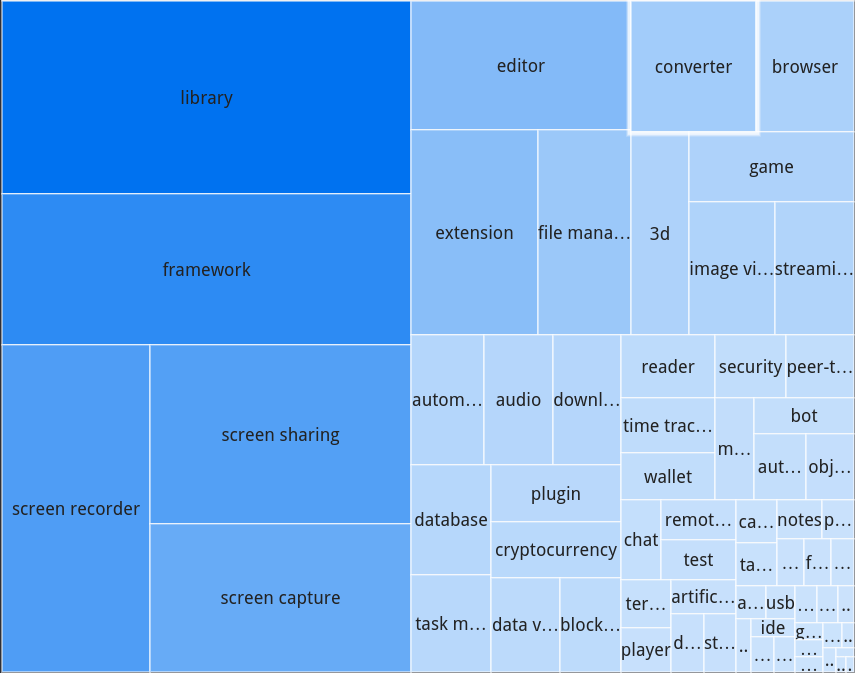
\includegraphics[width=0.9\textwidth]{images/dominios map.png}
    \caption{Percentual de RGDTEW para cada domínio}
    \label{fig:Percentual de repositórios por domínio}
\end{figure}
Dessa forma, com as métricas encontradas, é possível ver maior dominância dos domínios: \emph{Library} (Bibliotecas), \emph{Frameworks}, \emph{Screen Sharing}(Compartilhamento de tela), \emph{Screen recorder}(Gravador de tela), \emph{Screen capture}(Capturador de tela), \emph{Editor de texto}, \emph{Extension}(Extensões), \emph{File Management}(Gerenciador de Arquivos), \emph{Conversor}(Conversores), \emph{Browser}(Navegador).

\subsection{QP.2 A quantidade dos RGDTEW vem diminuindo ao longo da última década?}

Para a métrica M.3 (Média dos RGDTEW criados por ano para cada domínio), da QP.2, que consiste na média dos RGDTEW criados por ano para cada domínio, os resultados obtidos estão representados na Figura \ref{fig:10 domínios mais frequentes}, onde para efeito de melhor observabilidade foram selecionados apenas os 10 domínios mais frequentes.
\begin{figure}[ht]
    \centering
    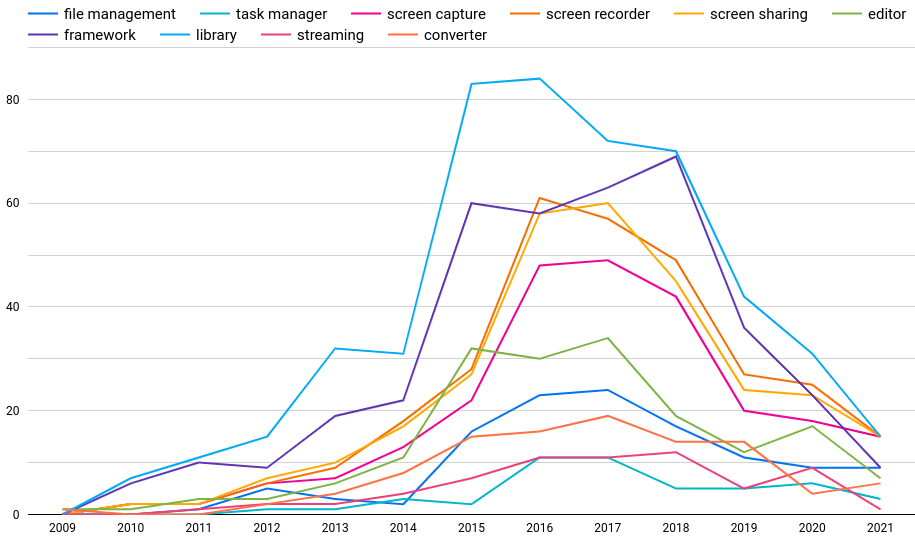
\includegraphics[width=1\textwidth]{images/10 dom mais fre.png}
    \caption{10 domínios mais frequentes}
    \label{fig:10 domínios mais frequentes}
\end{figure}
É possível observar na Figura \ref{fig:10 domínios mais frequentes} que houve um momento de pico na criação de RGDTEW no ano de 2016, seguido por uma queda o ano de 2021. 

Para a métrica M.4 (Média dos RGDTEW criados por ano), da QP.2, que consiste na média de repositórios com dependências de RGDTEW criados por ano, foram encontrados os resultados apresentados na Figura \ref{fig:RGDTEW criados de cada linguagem criados por ano}.
\begin{figure}[ht]
    \centering
    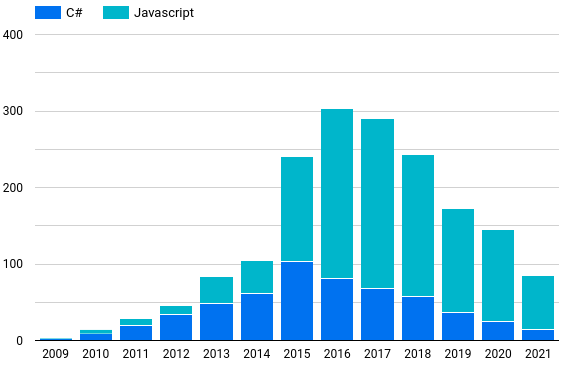
\includegraphics[width=0.9\textwidth]{images/lang por ano.png}
    \caption{RGDTEW criados de cada linguagem criados para cada ano}
    \label{fig:RGDTEW criados de cada linguagem criados por ano}
\end{figure}
Na Figura \ref{fig:RGDTEW criados de cada linguagem criados por ano} a evolução segue a mesma tendência da Figura \ref{fig:10 domínios mais frequentes}, pois estão diretamente relacionadas. Os repositórios da linguagem Javascript possuem maiores quantidades, pois representam a maioria dos repositórios coletados na pesquisa.

\subsection{QP.3 Os RGDTEW tem engajamento da comunidade?}

Para a métrica M.5 (Percentual de \emph{pull requests merged x not merged}), da QP.3, que consiste no percentual de \emph{pull Requests merged} e \emph{pull requests not merged}, os resultados obtidos são apresentados na Figura \ref{fig:Evolução dos Pull Requests por ano}. É possível observar o crescimento tanto dos \emph{pull requests merged} quanto dos  \emph{pull requests not merged}
\begin{figure}[ht]
    \centering
    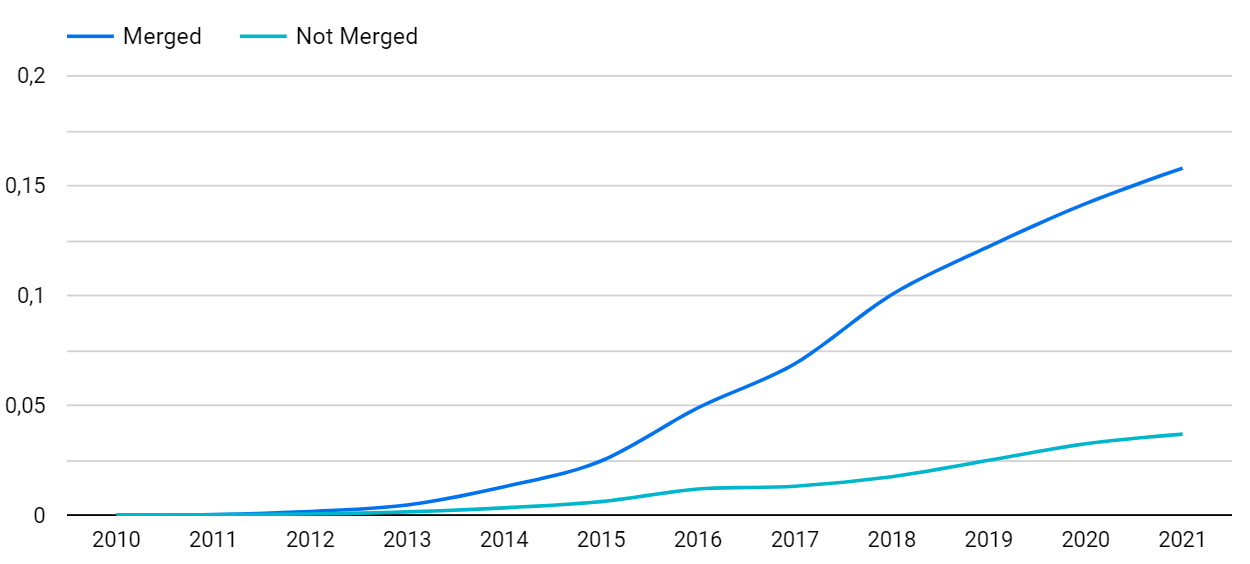
\includegraphics[width=0.9\textwidth]{images/percentual por ano PR.png}
    \caption{Evolução dos \emph{requests} por ano}
    \label{fig:Evolução dos Pull Requests por ano}
\end{figure}

Para a métrica M.6 (Percentual de \textit{issues} fechadas em relação a não fechadas dos RGDTEW por ano), da QP.3, o percentual de \emph{issues} fechadas e  \emph{issues} abertas, os resultados se encontram na Figura \ref{fig:Evolução das Issues por ano}.
\begin{figure}[ht]
    \centering
    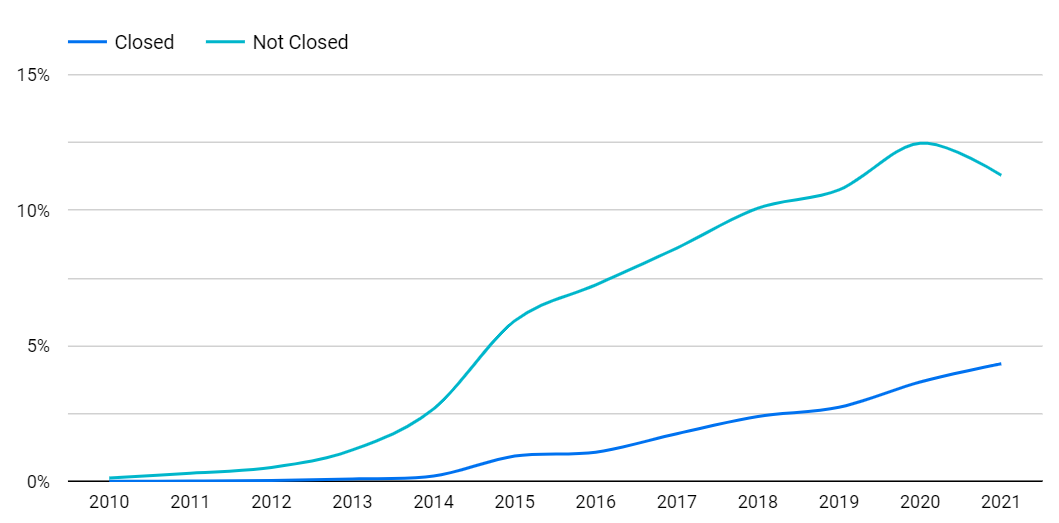
\includegraphics[width=0.9\textwidth]{images/issues por ano.png}
    \caption{Evolução das \emph{issues} por ano}
    \label{fig:Evolução das Issues por ano}
\end{figure}
Na Figura \ref{fig:Evolução das Issues por ano} nota-se que desde o começo da coleta, no ano de 2010, até o ano de 2020 as \emph{issues} fechadas cresceram em quantidade. Entretanto, após 2020, caíram. Já as \emph{issues} abertas, apresentaram crescimento em todo o percurso analisado. Sendo assim, é possível ver que existe um engajamento da comunidade considerando a diminuição de \emph{issues} abertas e \emph{pull requests merged}.

\section{Discussão} \label{discussao}

A busca dos repositórios, em um primeiro momento, retornou 1.781 resultados, como mostrado na Tabela \ref{tab:descricao x sem descricao}. Entretanto, 22,17\%, ou seja, 395 desses repositórios foram descartados por não possuir descrições para análise de domínio. Sendo assim, os resultados da pesquisa detiveram menos objetos de estudo do que o esperado inicialmente.

A categorização dos repositórios por domínio de aplicação, mostrado na Figura \ref{fig:Percentual de repositórios por domínio}, possibilita perceber quais são as mais frequentes aplicações criadas com  dependências do Electron e Windows Forms. Permitindo, dessa forma, cumprir o objetivo da pesquisa de caracterizar os repositórios com dependências \emph{desktop} e seus domínios. Além disso, também é possível visualizar os principais resultados na Figura \ref{fig:10 domínios mais frequentes}, tendo como domínios mais criados \emph{Library} e \emph{Framework}.

Como mostrado na Seção \ref{resultados}, a criação dos RGDTEW de 2009 a 2016 teve uma tendência de crescimento e no ano de 2016 teve seu ápice, nos anos seguintes, percebe-se uma mudança de tendência ocorrendo quedas consecutivas, como se vê na Figura \ref{fig:RGDTEW criados de cada linguagem criados por ano}. Entretanto, o engajamento da comunidade apresenta crescimento quando se analisa o percentual de \emph{pull requests merged} na Figura \ref{fig:Evolução dos Pull Requests por ano} e \emph{issues} fechadas na Figura \ref{fig:Evolução das Issues por ano}. Uma comunidade participativa contribui para a longevidade de uma aplicação dado que haverá mão de obra e conteúdo para resolver possíveis per causos durante a vida da aplicação.

\section{Ameaças à validade} \label{ameacas}

Pelo fato deste trabalho envolver diversas variáveis dependentes, como domínios datados automaticamente por inteligência artificial e quantidade de repositórios e seus respectivos engajamentos de \textit{pull requests} e \textit{issues}, além de variáveis independentes e controladas como as dependências Electron e Windows Forms. Com as decisões tomadas anteriormente definidas na \ref{metodologia} trazem para esse trabalho possíveis ameaças a validade deste estudo exploratório de caracterização dos domínios dos RGDTEW. Por meio da metodologia adotada, os passos foram feitos de forma que tais ameaças fossem mitigadas durante a execução da pesquisa e apresentado a quaisquer interessados na avaliação deste estudo.

Para cada tomada de decisão, foi analisada as possíveis ameaças. Diante disso, este processo possibilitou a identificação de ameaças à validade de conclusão. Devido ao fato da API do Github não fornecer uma forma nativa de buscar repositórios na linguagem JavaScript que possuem como dependência o \textit{framework} Electron, foi escolhido utilizar a ferramenta Selenium para criar um \emph{script} de automação de coleta dos repositórios no Github. Com isso, caso algum repositório Electron popular não tenha sido corretamente vinculado como dependente do Electron, não foi estudado nessa pesquisa. Outra ameaça a conclusão relacionada a API do \emph{Github}, é que também não é fornecida nativamente uma busca por repositórios C\# que possuem dependência da tecnologia de desenvolvimento \textit{desktop} \emph{Windows Forms}. O que também fez com que fosse escolhido utilizar o Selenium para mapear os repositórios e consequentemente podendo deixar algum repositório popular de fora do estudo.

Posteriormente, foi possível a ameaça à validade de construção, esta relacionada com a parcela de repositórios estudados nesta pesquisa. Isso, pois, os 1.386 repositórios com domínios definidos pode não ser equivalente a uma seleção maior de repositórios que dependem das tecnologias Electron e Windows Forms. Para mitigar este problema de generalização, foram escolhidos os repositórios mais populares conforme o número d estrelas.

No que tende ameaças à valida interna, foi detectada uma instabilidade com relação à ferramenta Selenium utilizada, pois, devido à quantidade de mais de 2 milhões de \textit{pull requests} e \textit{issues} buscados nesse trabalho, em alguns momentos a plataforma do Github barrava a conexão com as páginas. Desta forma, para mitigar, foi necessário implementar um sistema para aguardar alguns minutos até que conexão fosse liberada. Diante disso, caso ocorresse alguma atualização nas \textit{pull requests} e \textit{issues} do repositório, há chances de não estarem datadas na paginação feita na busca de dados. Outra ameaça interna que vale ressaltar, é o não controle total do retorno da inteligência artificial da OpenAI, que para um mesmo repositório, pode classificar de formas diferentes os domínios, porém, com o mesmo objetivo final, basicamente mudando apenas palavras e formas de expressão. Para mitigar este problema, foi foram feitas duas classificações utilizando a inteligência artificial, uma primeira para gerar os prováveis domínios dos repositórios e uma segunda, reclassificando em domínios manualmente filtrados.

Por fim, foi identificado a ameça à validade externa que a análise desta pesquisa foi feita com 1.781 RGDTEW, contudo, apenas 1.386 repositórios foi possível definir domínios, devido à falta de descrições bem elaborados por parte dos criadores dos repositórios e limitações da inteligência artificial da OpenAI. Para mitigar esta ameaça, como explicado na \ref{metodologia}, foi feita uma análise e seleção manual de domínios a partir da primeira lista de domínios classificados pela inteligência artificial. Além disso, todos os repositórios com domínios passaram por uma segunda classificação dos domínios baseados nos domínios filtrados manualmente, por meio novamente da OpenAI, para diminuir as variações e garantir com maior precisão quais os domínios de cada repositório.

\section{Conclusão} \label{conclusao}

Nesse trabalho, foram analisados os repositórios mais populares dependentes das tecnologias Electron e Windows Forms ao longo dos últimos dez anos, visando identificar os principais domínios atualmente e ao longo do tempo. Além disso, visa identificar as tendências de crescimento engajamento da comunidade desses repositórios ao longo dos anos. 

Foi possível identificar que os principais domínios desses repositórios são  \textit{Library} e \textit{Framework}, seguidos dos domínios relacionados a captura de imagem de tela (\textit{Screen Recorder}, \textit{Screen Sharing} e \textit{Screen Capture}) e editores. Foi possível identificar também que o número de repositórios vêm diminuindo nos últimos anos, e teve seu pico em 2016. Em contrapartida, o engajamento da comunidade tem apresentado crescimento ao longo dos anos.

Como trabalhos futuros, seria relevante fazer a mesma análise para um contexto mais amplo. Um exemplo seria avaliar outros \textit{frameworks} e bibliotecas de outras linguagens usadas para a construção de aplicações desktop.

\bibliographystyle{sbc}
\bibliography{sbc-template}

\end{document}
